\documentclass{beamer}
\usepackage[utf8]{inputenc}
\usepackage{listings}
\usepackage{graphicx}
\usetheme{Madrid}
\usecolortheme{beaver}

\input{revision}

\title{Elixir and Erlang tests}
\subtitle{Baby steps}
\author[joaohf]{João Henrique Ferreira de Freitas \\ \texttt{https://github.com/joaohf} \\ \texttt{joaof@gmail.com}}
\date[EMC 2018]{Elixir Meetup, Campinas 2018}

\logo{\Revision}

%\AtBeginSection[]
%{
%  \begin{frame}
%    \frametitle{Table of Contents}
%    \tableofcontents[currentsection]
%  \end{frame}
%}

\begin{document}
  \begin{frame}
    \titlepage
  \end{frame}

  \section[Section]{Types of tests}
  
  \begin{frame}
    \frametitle{Types of tests}   
    \begin{itemize}
      \item <1-> Unit
      \item <2-> Integration
      \item <3-> Functional    
    \end{itemize}
  \end{frame}
  
  \begin{frame}
    \frametitle{Examples}
    \framesubtitle{Unit}

    \begin{block}{}      
    What is a unit? \pause
    \end{block}
    
    \begin{alertblock}{}
    A function/method, class, module. Usually a unit is a independent peace of code.
    \end{alertblock}
    
  \end{frame}
  
  \begin{frame}[fragile]
    \frametitle{Examples}
    \framesubtitle{Unit}
    
    \begin{lstlisting}[]
    defmodule ExServer do
    def f(x) when is_integer(x) do  
      true
    end
    def f(x) when is_binary(x) do
      true
    end
    end
    \end{lstlisting}
  \end{frame}
  
  \begin{frame}
    \frametitle{Examples}
    \framesubtitle{Integration}
    
    \begin{block}{}      
    What does a integration? \pause
    \end{block}
    
    \begin{alertblock}{}
    Test how parts of the system work together.
    \end{alertblock}
    
    \begin{examples}
    \begin{itemize}
    \item Databases
    \item Message Queues
    \item Network operations
    \item Other systems    
    \end{itemize}

    \end{examples}
        
  \end{frame}
  
  \begin{frame}
    \frametitle{Examples}
    \framesubtitle{Integration}
    
    \begin{figure}[t]
    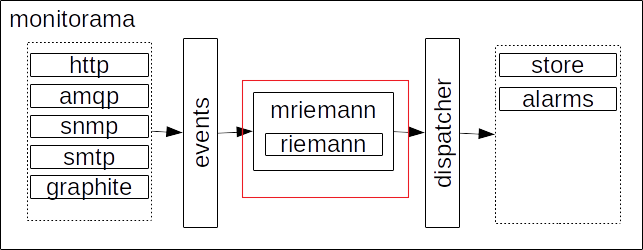
\includegraphics[scale=0.5]{img/ex1.png}
    \centering
    \end{figure}
    
  \end{frame}

  \begin{frame}
    \frametitle{Examples}
    \framesubtitle{Functional}
    
    \begin{block}{}      
    That's the E2E tests? \pause
    \end{block}
    
    \begin{alertblock}{}
    Tests that simulates real users and operations.
    \end{alertblock}
        
  \end{frame}
  
  \begin{frame}
    \frametitle{Examples}
    \framesubtitle{Functional}
    
    \begin{figure}[t]
    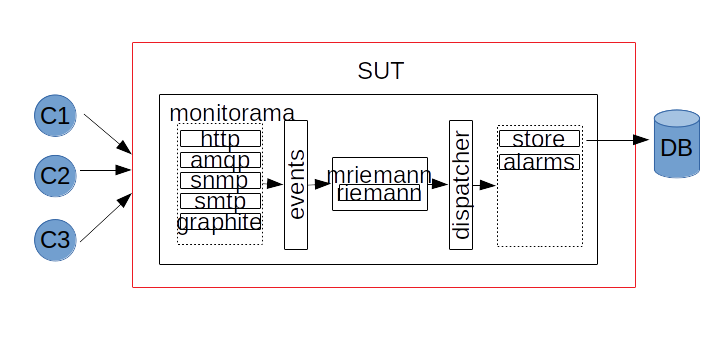
\includegraphics[scale=0.5]{img/ex2.png}
    \centering
    \end{figure}
    
  \end{frame}

  \subsection[Section]{Tools}
      
  \begin{frame}
    \frametitle{Tools}
    \framesubtitle{}
    
    \begin{itemize}[<+->]
    \item Erlang and Elixir has strong tools to do all kind of tests
    \item Mainly integrated with tooling like mix or rebar3
    \item Is straightforward    
    \end{itemize}
  \end{frame}
  
  \begin{frame}
    \frametitle{Tools}
    \framesubtitle{Erlang}
    
    To code:
    \begin{itemize}[<+->]
    \item \href{http://erlang.org/doc/apps/eunit/chapter.html}{eunit}
    \item \href{http://erlang.org/doc/apps/common_test/introduction.html}{Common Test}
    \end{itemize}
    To see coverage:
    \begin{itemize}[<+->]
    \item \href{http://erlang.org/doc/apps/tools/cover_chapter.html}{cover}
    \end{itemize}
    Any additional tools?
    \begin{itemize}[<+->]
    \item \href{https://github.com/eproxus/meck}{meck}
    \item \href{http://proper.softlab.ntua.gr}{proper}
    \item \href{http://www.quviq.com/downloads}{QuickCheck}
    \end{itemize}    
  \end{frame}
    
  \begin{frame}
    \frametitle{Tools}
    \framesubtitle{Elixir}
    
    To code:
    \begin{itemize}[<+->]
    \item \href{https://hexdocs.pm/ex_unit/ExUnit.html}{ExUnit}
    \item \href{https://hexdocs.pm/ex_unit/ExUnit.DocTest.html}{doctest}
    \end{itemize}
    To see coverage:
    \begin{itemize}[<+->]
    \item \href{http://erlang.org/doc/apps/tools/cover_chapter.html}{cover, mix test}
    \end{itemize}
    Any additional tools?
    \begin{itemize}[<+->]
    \item \href{https://github.com/plataformatec/mox}{mox}
    \item \href{https://elixir-lang.org/blog/2017/10/31/stream-data-property-based-testing-and-data-generation-for-elixir}{StreamData: Property-based testing}
    \item \href{http://www.quviq.com/downloads/}{QuickCheck}
    \end{itemize}    
  \end{frame}  

  \begin{frame}
    \frametitle{Stop the world!}
    \framesubtitle{What is proper testing?}
    
    
  \end{frame}

  \begin{frame}
    \begin{center}
    \Huge Thank You!
    \end{center}
  \end{frame}
    
  \begin{frame}
    \frametitle{Colophon}
    
    \begin{itemize}
    \item Latex
    \item Beamer
    \item Texmaker
    \end{itemize}
    
  \end{frame}
  
  
  
% etc
\end{document}
